\apendice{Plan de Proyecto Software}\label{anex:A}

\section{Introducción}

Lo primero que se debería hacer al iniciar un proyecto y antes de comenzar con el desarrollo es la planificación del mismo. Es necesario realizar una estimación de coste en tiempo y dinero que nos va a suponer realizar el proyecto y una vez conozcamos esta estimación deducir si el proyecto se puede realizar exitosamente o no. 
Para realizar esta tarea en este documento vamos a realizar dos tareas:

\begin{description}
	\tightlist
	\item[Planificación temporal.] Donde estimaremos el tiempo que requiere la realización del proyecto.
	\item[Estudio de la viabilidad.] Donde se deduce si el proyecto es viable, tanto económica como legalmente: 
	\begin{description}
		\tightlist
		\item[Viabilidad económica.] Se estudia el coste que supondría haber realizado el proyecto en un entorno real y se analizan posibles maneras de monetizar el proyecto para cubrir este coste.
		\item[Viabilidad legal.] Se estudian las leyes aplicables al proyecto y los aspectos más relevantes a nivel legal.
	\end{description}
\end{description}

\section{Planificación temporal}

Se ha optado por la metodología \textbf{SCRUM} \cite{scrum_master_scrum_2019}, donde se trabaja con un ciclo de vida que se repite durante el proyecto. Trabajar con esta metodología ha significado que:
\begin{itemize}
	\item Se ha trabajado de manera incremental y evolutiva.
	\item Se han trabajado en iteraciones (llamados \textit{sprints} en la metodología \textbf{\textit{SCRUM}}) de dos semanas. Estos \textit{sprints} finalizan con una reunión entre el tutor y alumno donde:
	\begin{itemize}
		\item Se llevaba a cabo la \textit{sprint review}, donde se revisa el trabajo realizado durante el \textit{sprint} que finaliza y se tratan los avances realizados así como los problemas con los que el alumno se ha encontrado.
				\item Una segunda parte donde se lleva a cabo la \textit{sprint planning}, donde se planifica el trabajo a realizar durante el siguiente \textit{sprint} planteando tareas y seleccionándolas del \textit{product backlog}, pasándolas a la pila de trabajo del \textit{sprint} que comienza, el \textit{sprint backlog}.\\
				Estas tareas se han registrado en el sistema de gestión de incidencias de \textit{GitHub} , \textit{GitHub Issues} \footnote{Planificación de proyectos para desarrolladores - \url{https://github.com/features/issues}} y el trabajo con \textit{sprints} se ha llevado a cabo a través de \textit{ZenHub} \footnote{Página de inicio de \textit{ZenHub} - \url{https://www.zenhub.com/}} integrado directamente en \textit{GitHub}.
	\end{itemize}
\end{itemize}

\subsection{\textit{Sprints} realizados}

Además de la división del desarrollo del proyecto en \textit{sprints}, podemos dividirlo en diferentes fases:


\begin{itemize}
	\item Durante la primera fase se llevaron a cabo tareas de \textbf{investigación} y \textbf{estudio} del proyecto previo\cite{TFGPrevio} así como de las bases teóricas y herramientas que se utilizarían durante el proceso.
	
	\item En la segunda fase, una vez comprendidos los conceptos planteados en el proyecto ya existente y en las bases teóricas (métricas, \textit{framework}  de medición, estructura del proyecto, etc.) se realizaron tareas de \textbf{configuración} del entorno de desarrollo, tanto para el código como para la memoria del proyecto.
	
	\item Tercera fase donde gracias a la investigación y estudio realizados se realizan diferentes tareas de \textbf{documentación} de la memoria del proyecto.
	
	\item Cuarta fase, la más extensa de todas, donde se realizan tareas de \textbf{desarrollo} para actualizar las dependencias del proyecto, implementar nuevas métricas, mejoras en la interfaz y la integración con \textit{GitHub}.
	
	\item Quinta fase final de \textbf{documentación} en la que se finaliza la memoria y se trabaja en los anexos. Finalmente se preparan los vídeos necesarios y las guías de usuario.
\end{itemize}

En la siguiente sección se van a describir estas fases, que se pueden también consultar a través de las \textit{issues} del repositorio del proyecto:\\

\url{https://github.com/Joaquin-GM/GII_O_MA_19.07-Comparador-de-metricas-de-evolucion-en-repositorios-Software} \\

Se utilizarán de manera explicativa capturas de la gestión de los \textit{sprints} gestionados con \textit{ZenHub}.



\subsubsection{Investigación y estudio}

Esta fase inicial comenzó en octubre de 2021 y duró aproximadamente 3 \textit{sprints} (6 semanas) durante los que se asentó la base teórica del proyecto y se comprendió la estructura del mismo así como los objetivos. Además del trabajo con las referencias teóricas como \cite{ratzinger_space:_2007} se buscó información sobre trabajos y aplicaciones que están relacionados con la temática de este proyecto ya entreviéndose que hay muy pocas soluciones similares y ninguna con las capacidades que tendría el proyecto a su finalización.\\
También se realizó la formación en \textit{Vaadin} que proponen los propios creadores del \textit{framework} \footnote{Centro de aprendizaje de \textit{Vaadin} - \url{https://vaadin.com/learn/tutorials?version=v14}} así como tutoriales para que el alumno se familiarizara con \textit{LaTeX} y con la herramienta utilizada \textit{TexMaker}\footnote{\textit{TexMaker} editor \textit{LaTeX} - \url{https://www.xm1math.net/texmaker/}}.\\

A continuación se muestran algunas de las \textit{issues} con las que se trabajó en esta fase:

\begin{figure}[!h]
	\centering
	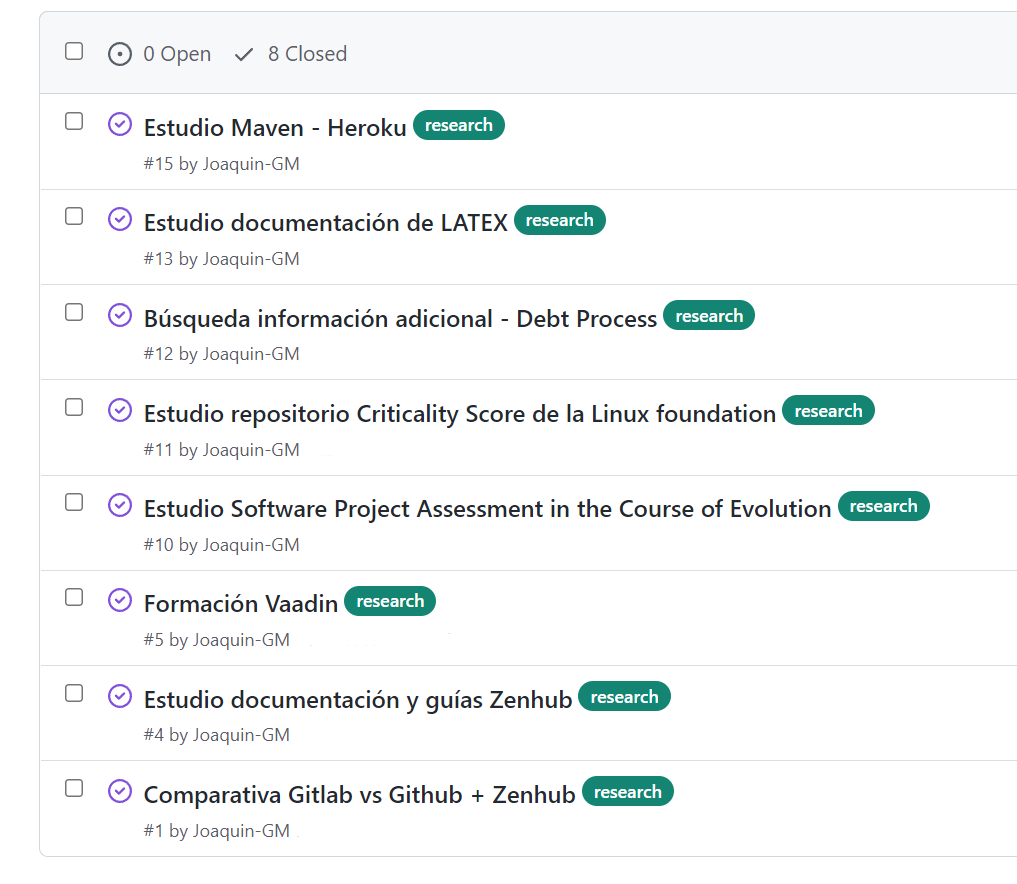
\includegraphics[scale=0.50]{AnexA_Research_Issues}
	\caption{\textit{Issues} relacionadas con la fase de estudio e investigación investigación}
	\label{fig:AnexA_Research_Issues}
\end{figure}
\FloatBarrier

\subsubsection{Configuración del entorno de desarrollo}

En esta fase se trabajó configurando las diferentes herramientas que se iban a utilizar en el proyecto, \textit{GitHub} + \textit{ZenHub} para la gestión de \textit{issues} y \textit{sprints}, Eclipse como \textit{IDE} de desarrollo, \textit{Maven} y \textit{Jetty} para la gestión y ejecución del proyecto en local y \textit{TexMaker} como editor \textit{LaTeX} para trabajar con la memoria. Esta fase duró otros tres \textit{sprints} (6 semanas) y a continuación se muestran las las \textit{issues} con las que se trabajó en esta fase:

\begin{figure}[!h]
	\centering
	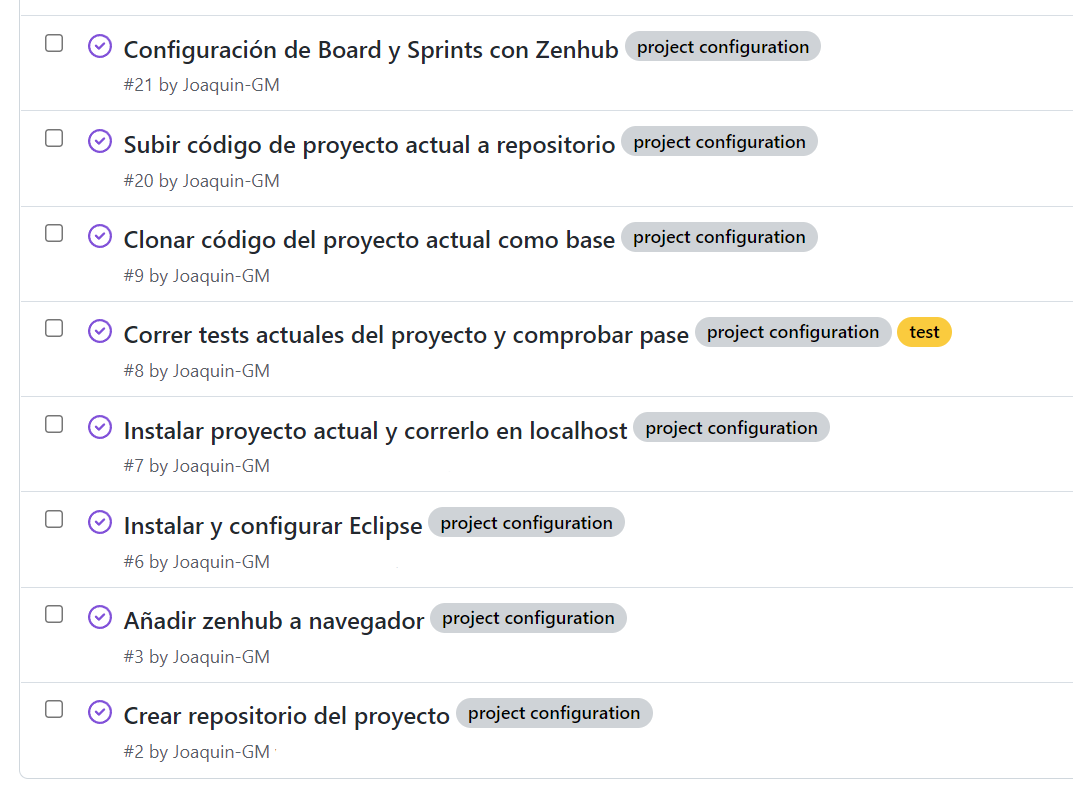
\includegraphics[scale=0.50]{AnexA_Configuration_Issues}
	\caption{\textit{Board} del proyecto en \textit{ZenHub}}
	\label{fig:AnexA_Configuration_Issues}
\end{figure}
\FloatBarrier

También se muestra en la figura \ref{fig:AnexA_Zenhub_Board} cómo quedó el tablero de \textit{ZenHub} una vez estuvo integrado en el repositorio directamente en \textit{GitHub} a través de la extensión de navegador de \textit{ZenHub}:

\begin{figure}[!h]
	\centering
	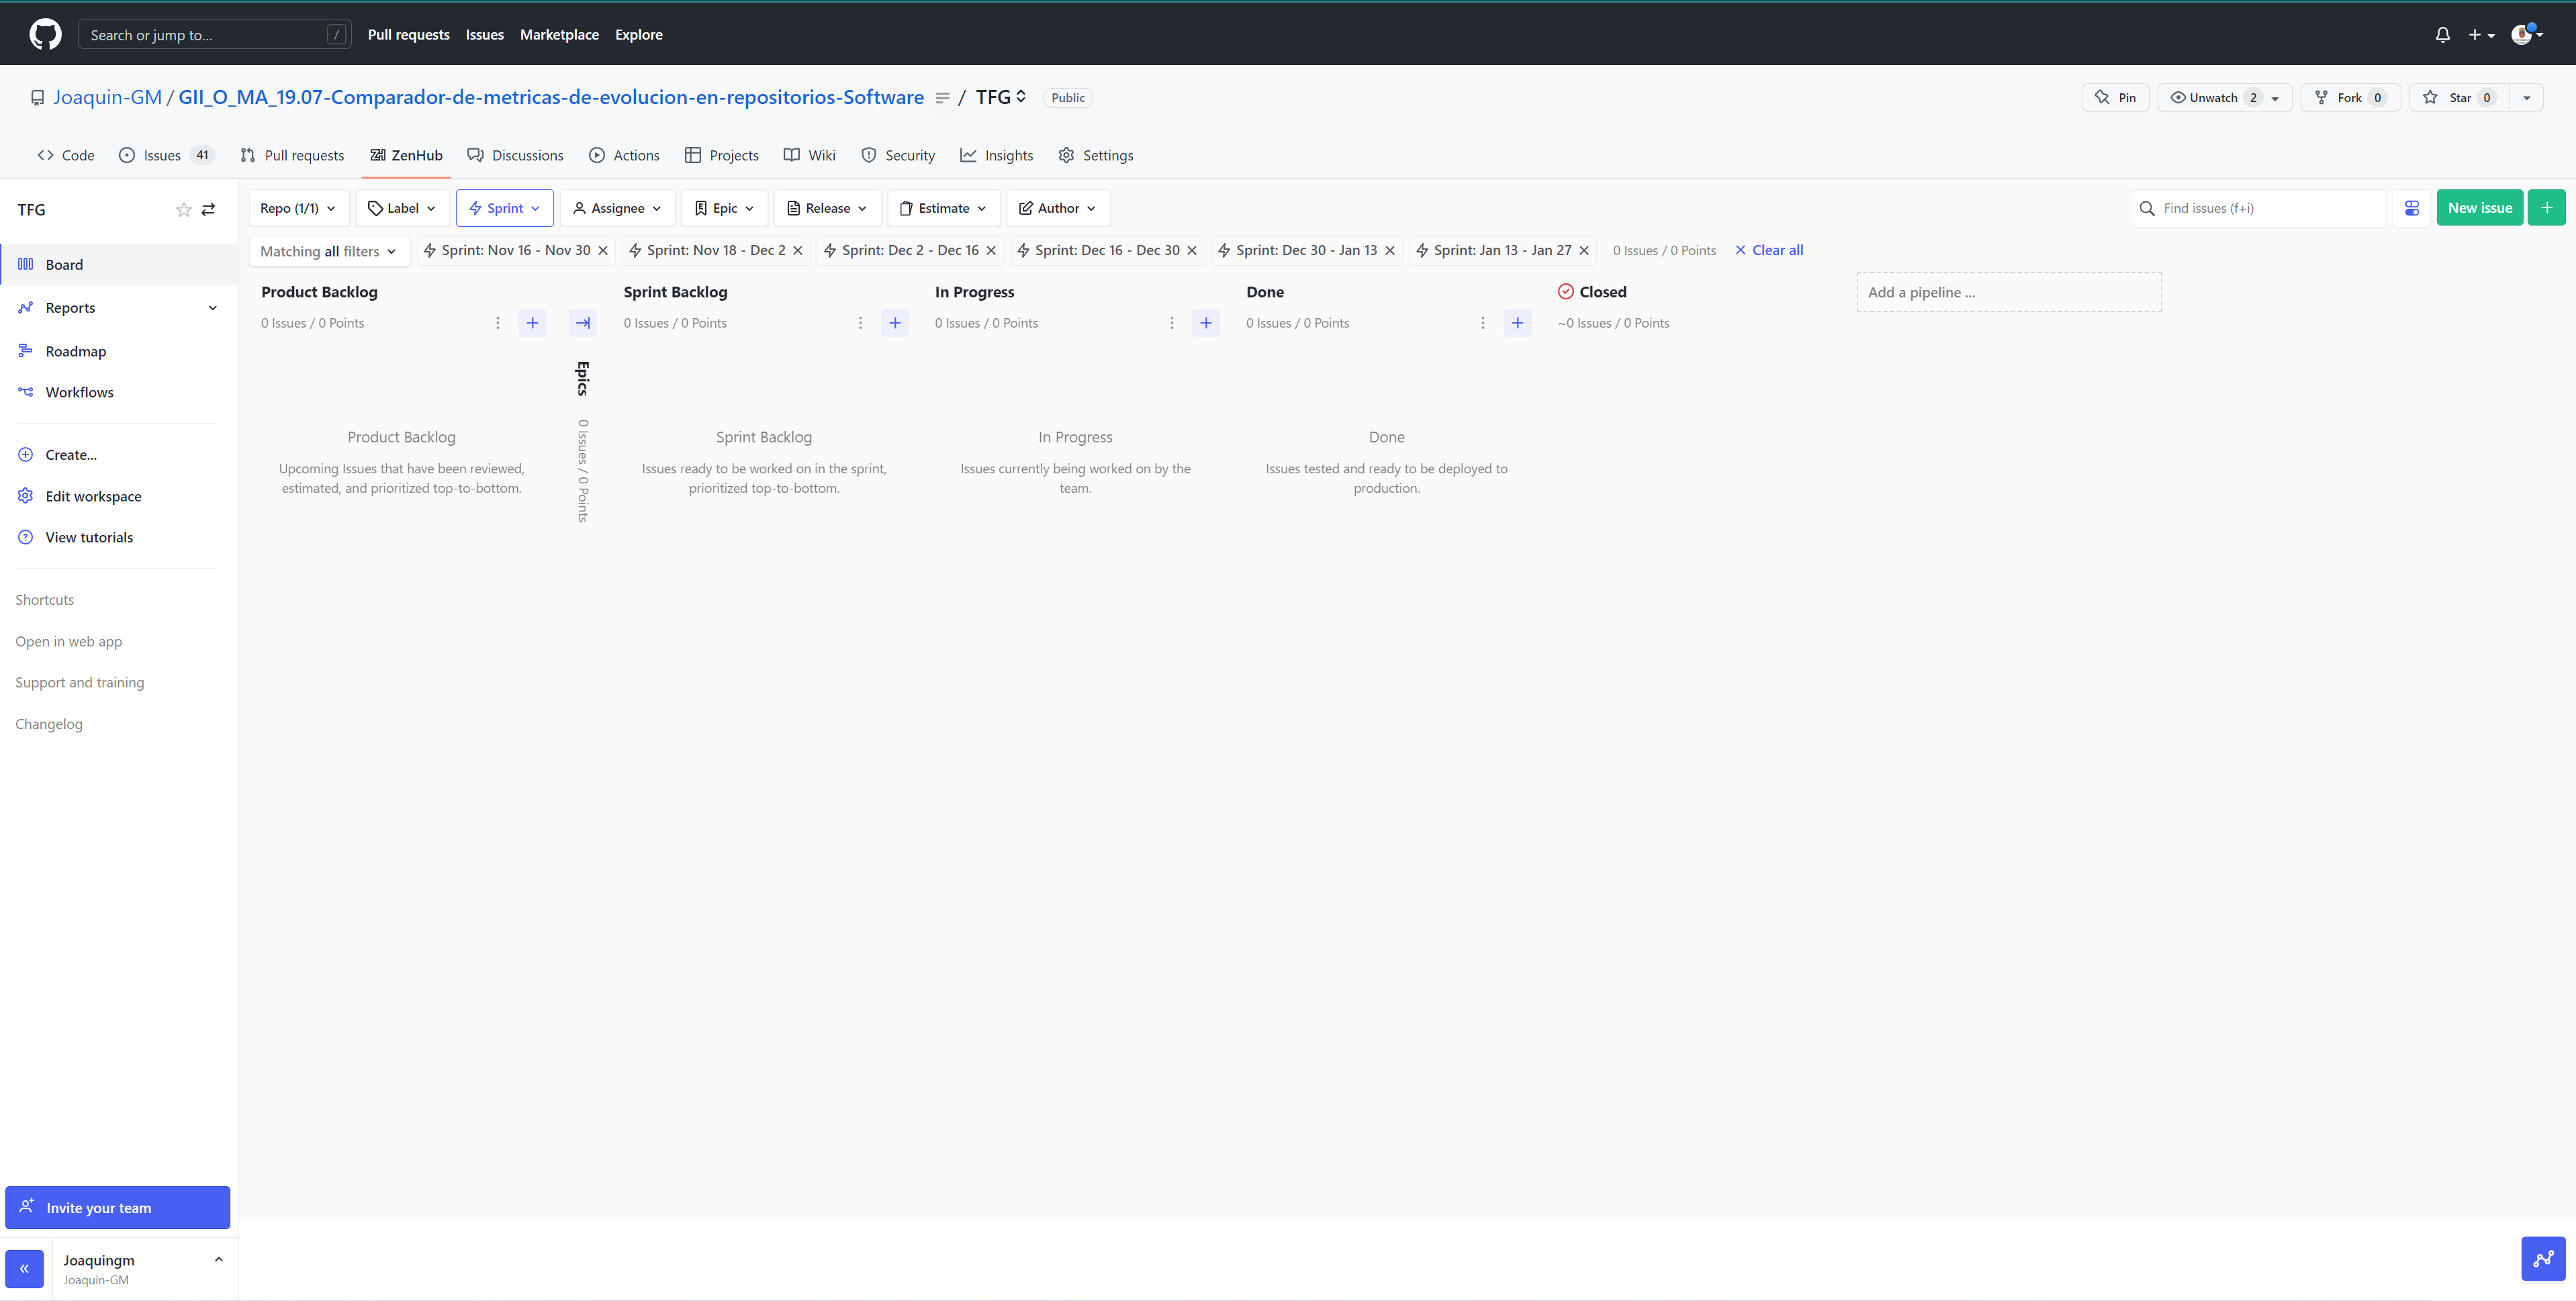
\includegraphics[width=1\textwidth]{AnexA_Zenhub_Board}
	\caption{Creación de nueva \textit{issue} en \textit{ZenHub}}
	\label{fig:AnexA_Zenhub_Board}
\end{figure}
\FloatBarrier

Como se puede apreciar en la figura anterior, \textit{ZenHub} provee de numeras herramientas muy útiles para la gestión de las \textit{issues} del proyecto permitiéndonos trabajar con ellas de forma sencilla y agruparlas en \textit{sprints}.\\
Para facilitar la creación de nuevas \textit{issues} se crearon plantillas que se pueden utilizar también desde el menú de creación de \textit{issues} de \textit{ZenHub}:

\begin{figure}[!h]
	\centering
	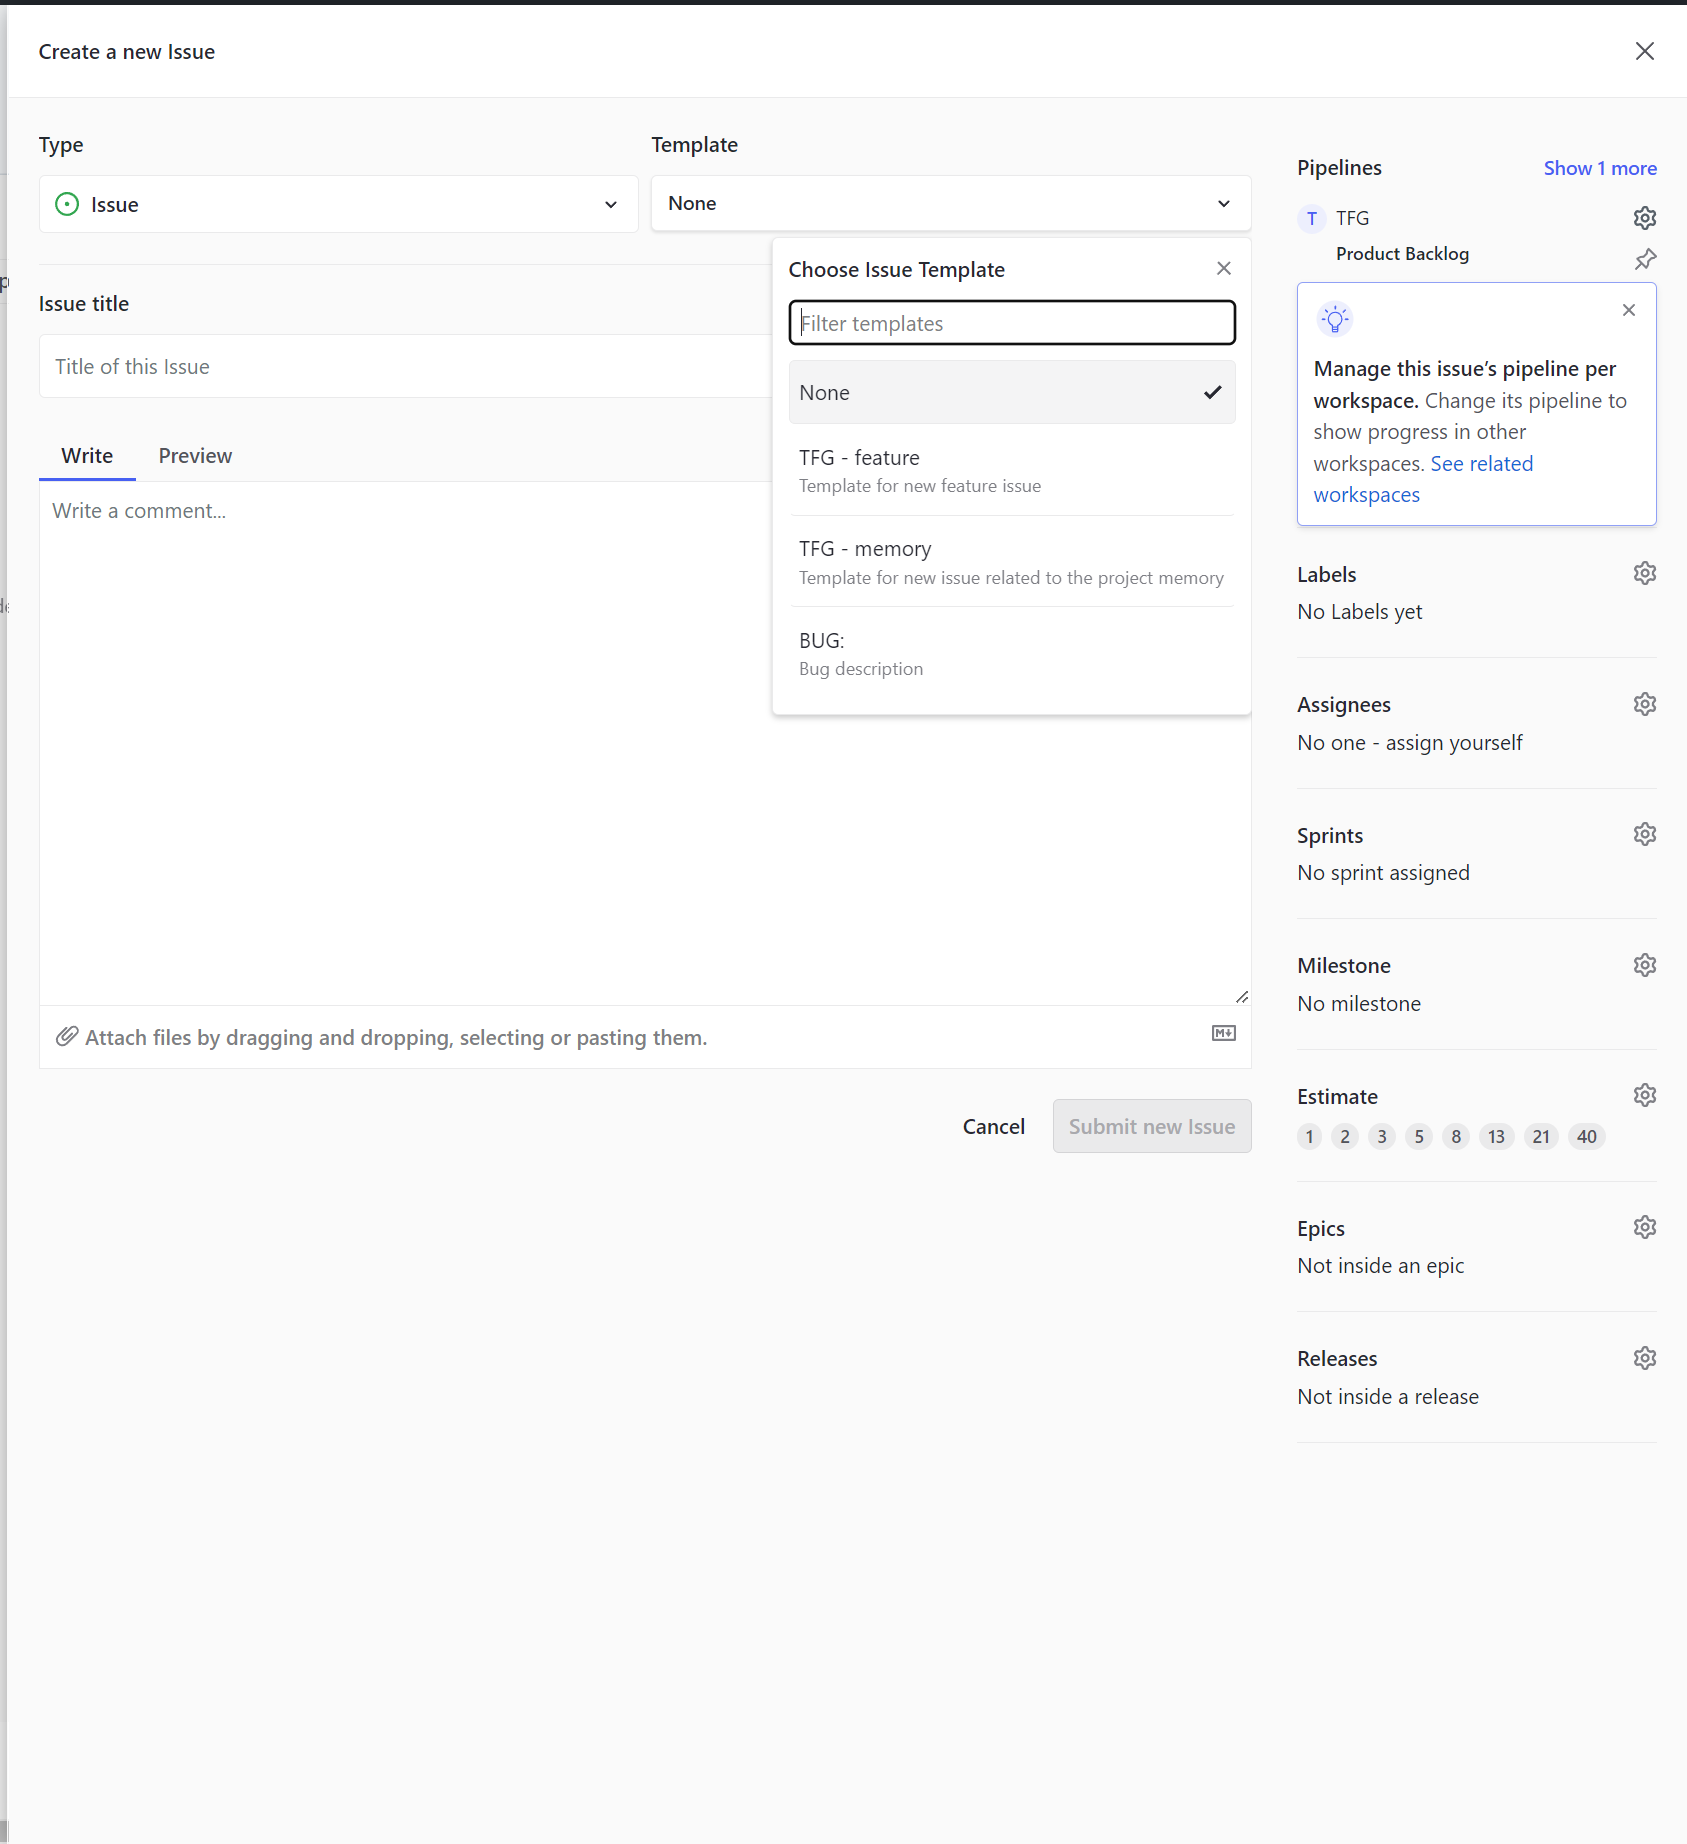
\includegraphics[width=1\textwidth]{AnexA_Zenhub_Create_New_Issue}
	\caption{Creación de nueva \textit{issue} en \textit{ZenHub}}
	\label{fig:AnexA_Zenhub_Create_New_Issue}
\end{figure}
\FloatBarrier

\subsubsection{Primera fase de documentación}

En esta primera fase de documentación se trabajó durante 3 \textit{sprints} (6 semanas) en los siguientes apartados de la memoria:

\begin{itemize}
	\item Introducción y Objetivos
	\item Resumen y Descriptores
	\item Conceptos teóricos
	\item Técnicas y herramientas
	\item Aspectos relevantes del desarrollo del proyecto (que se finalizaría más adelante)
\end{itemize}

A continuación podemos ver las \textit{issues} con las que se trabajó en esta fase:

\begin{figure}[!h]
	\centering
	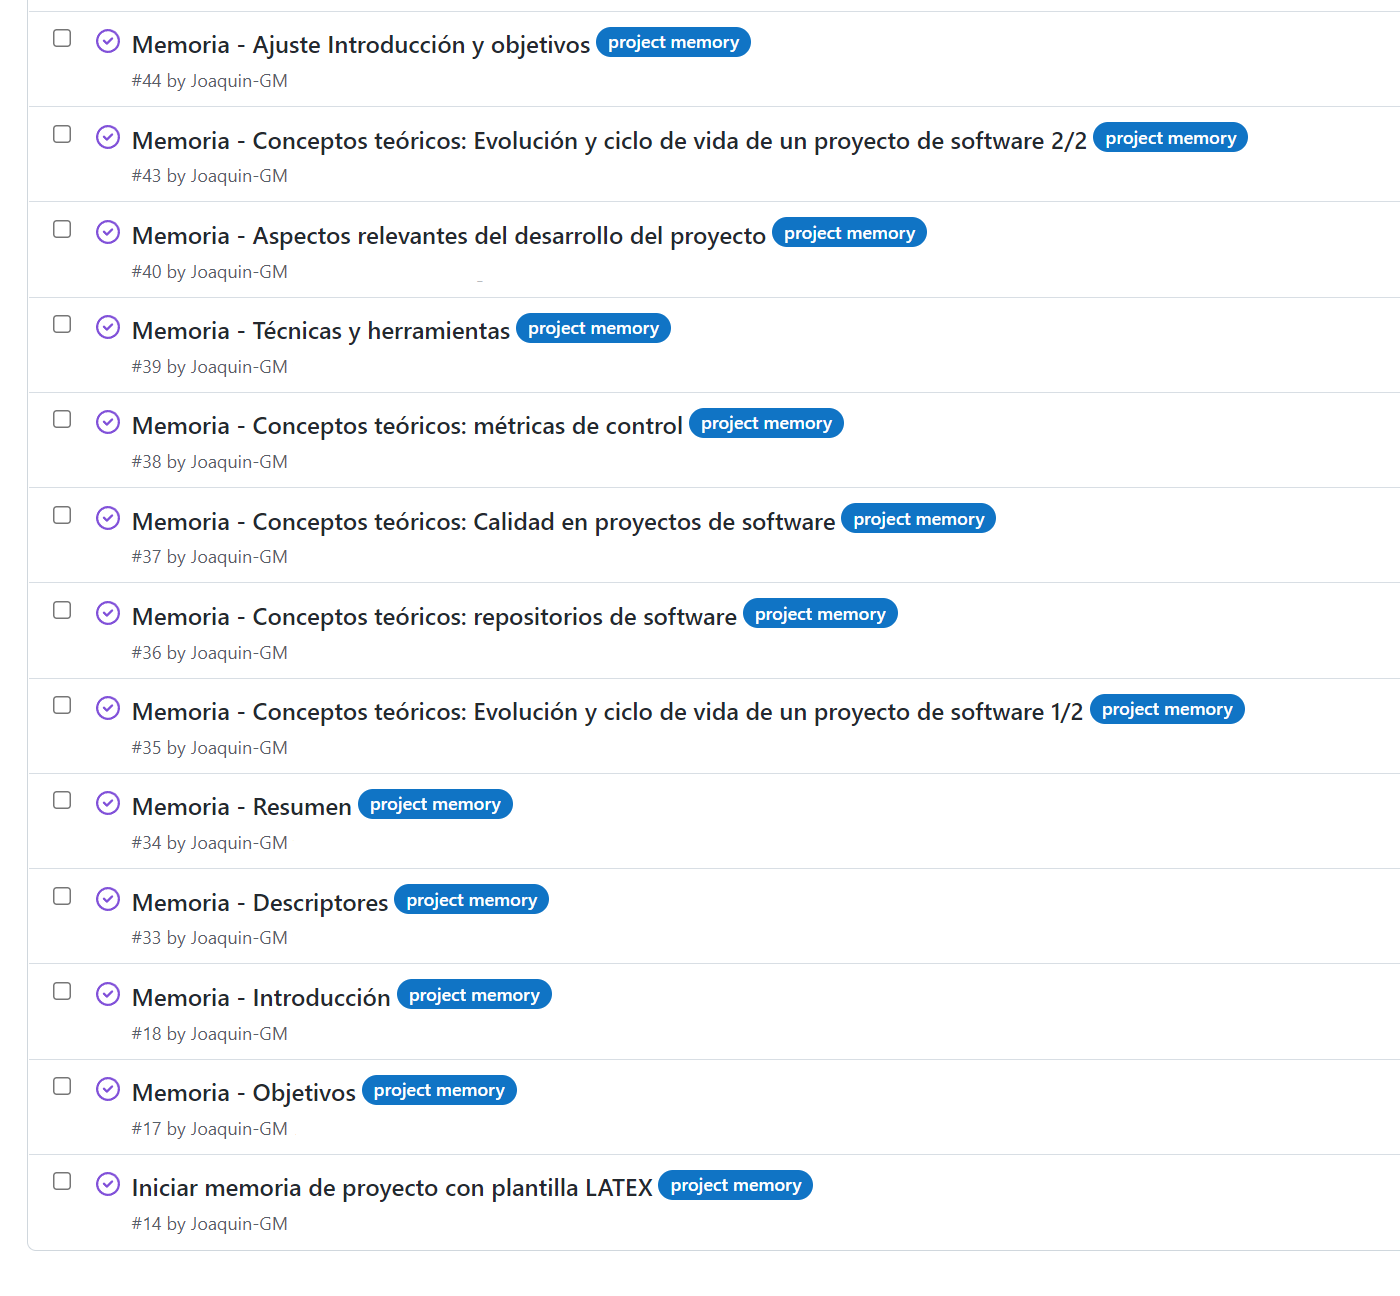
\includegraphics[width=1\textwidth]{AnexA_First_Memory_Issues}
	\caption{Primeras \textit{issues} relacionadas con la memoria}
	\label{fig:AnexA_First_Memory_Issues}
\end{figure}
\FloatBarrier

\textit{ZenHub} también nos proporciona información sobre la gestión de las \textit{issues} y el avance del proyecto. Podemos destacar los gráficos \textit{burndown} que representan el avance durante el transcurso del sprint, marcando una guía orientativa de cómo debería ser. Este tipo de gráfico representa los puntos asignados a las diferentes \textit{issues} y va bajando conforme éstas se van cerrando durante el \textit{sprint}. \\
Como vemos en la figura \ref{fig:AnexA_First_Memory_BurnDown}, en algunos \textit{sprints} se estimó demasiado trabajo o bien no se pudo realizar al completo y en el siguiente gráfico se puede ver cómo no se llegan a completar todos los puntos de las \textit{issues} planteadas:

\begin{figure}[!h]
	\centering
	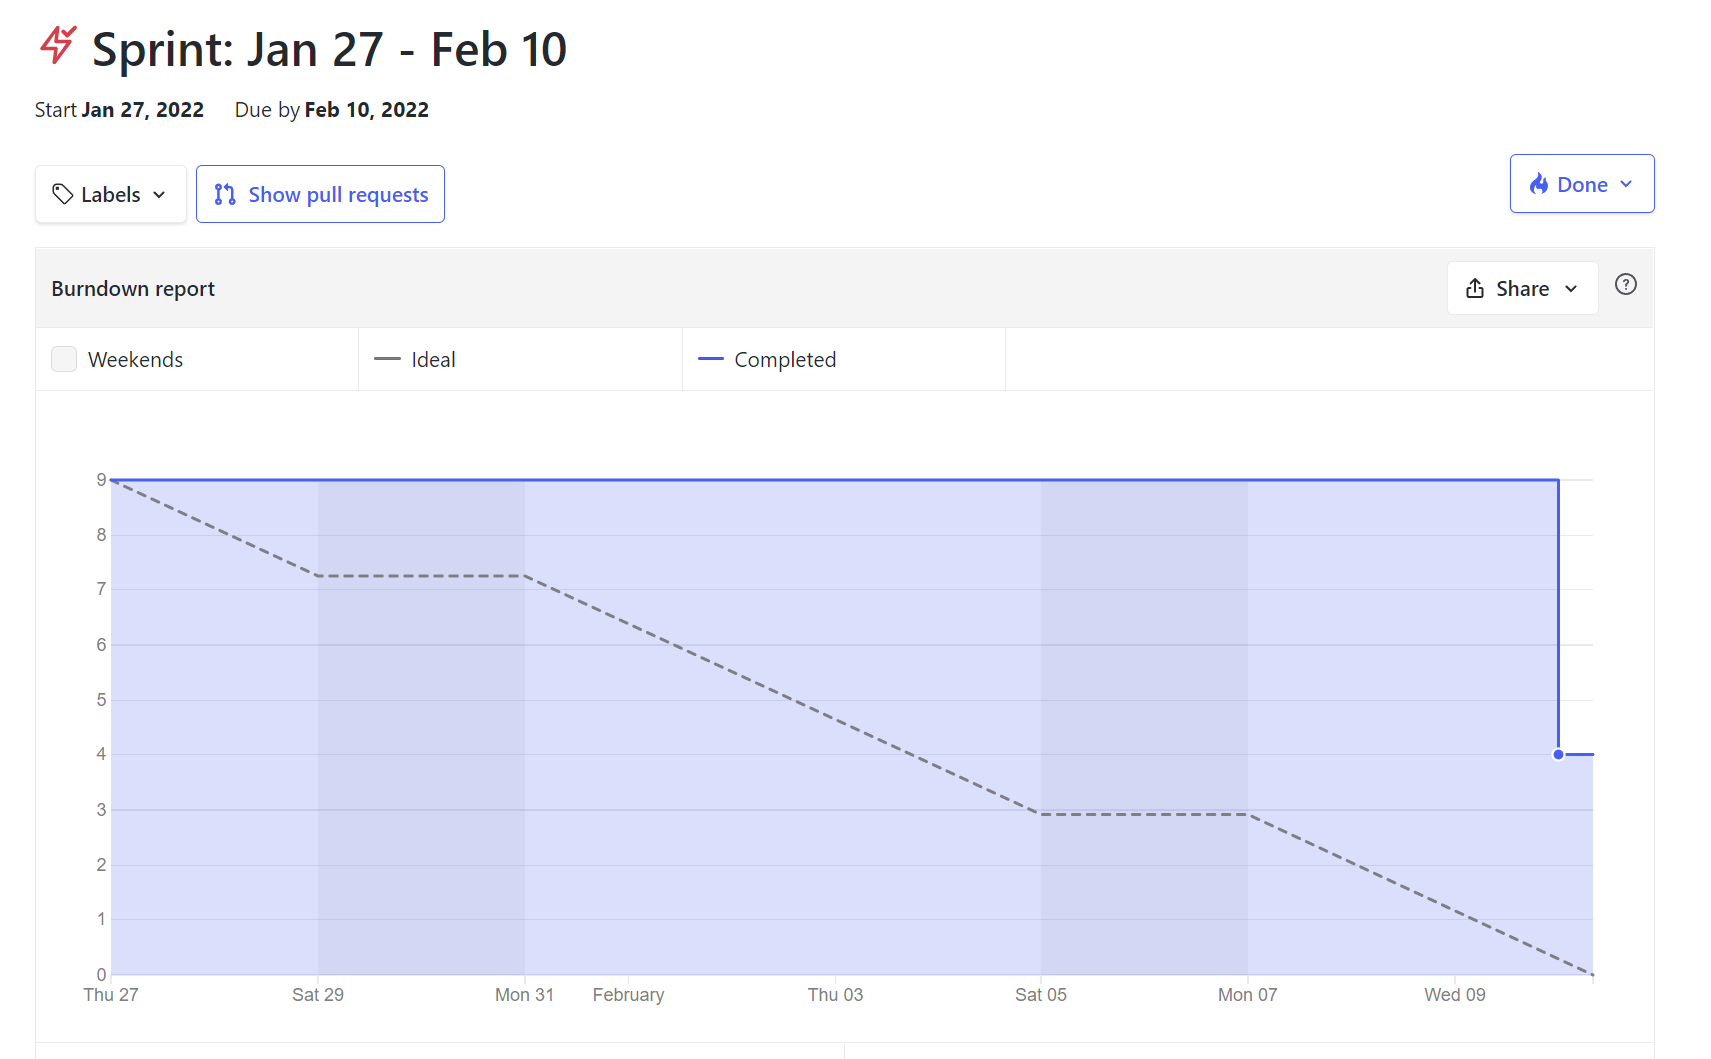
\includegraphics[width=1\textwidth]{AnexA_First_Memory_BurnDown}
	\caption{Primeras \textit{issues} relacionadas con la memoria}
	\label{fig:AnexA_First_Memory_BurnDown}
\end{figure}
\FloatBarrier

\subsubsection{Fase de implementación de mejoras y nueva funcionalidad}
La más larga de todas las fases con una duración de unos 7 \textit{sprints} (14 semanas). En esta fase se realizaron las tareas de desarrollo entre las que destacan:

\begin{itemize}
	\item Actualización del código previo y dependencias.
	\item Corrección de \textit{bugs}  existentes.
	\item Mejora del motor de cálculo de métricas para casos poco comunes.
	\item Mejoras de interfaz y usabilidad (leyenda, tooltips, separación por grupos de métricas, botones para cerrar diálogos, etc.)
	\item Nuevas métricas \textit{CICD}: IC1, IC2, IC3, P1 y P2
	\item Adaptación de las funcionalidades a las nuevas métricas (export, import, actualización, etc.)
	\item Integración con \textit{GitHub} y adaptación de la interfaz.
\end{itemize}

Las \textit{issues} que se han realizado en esta fase son:

\begin{figure}[!h]
	\centering
	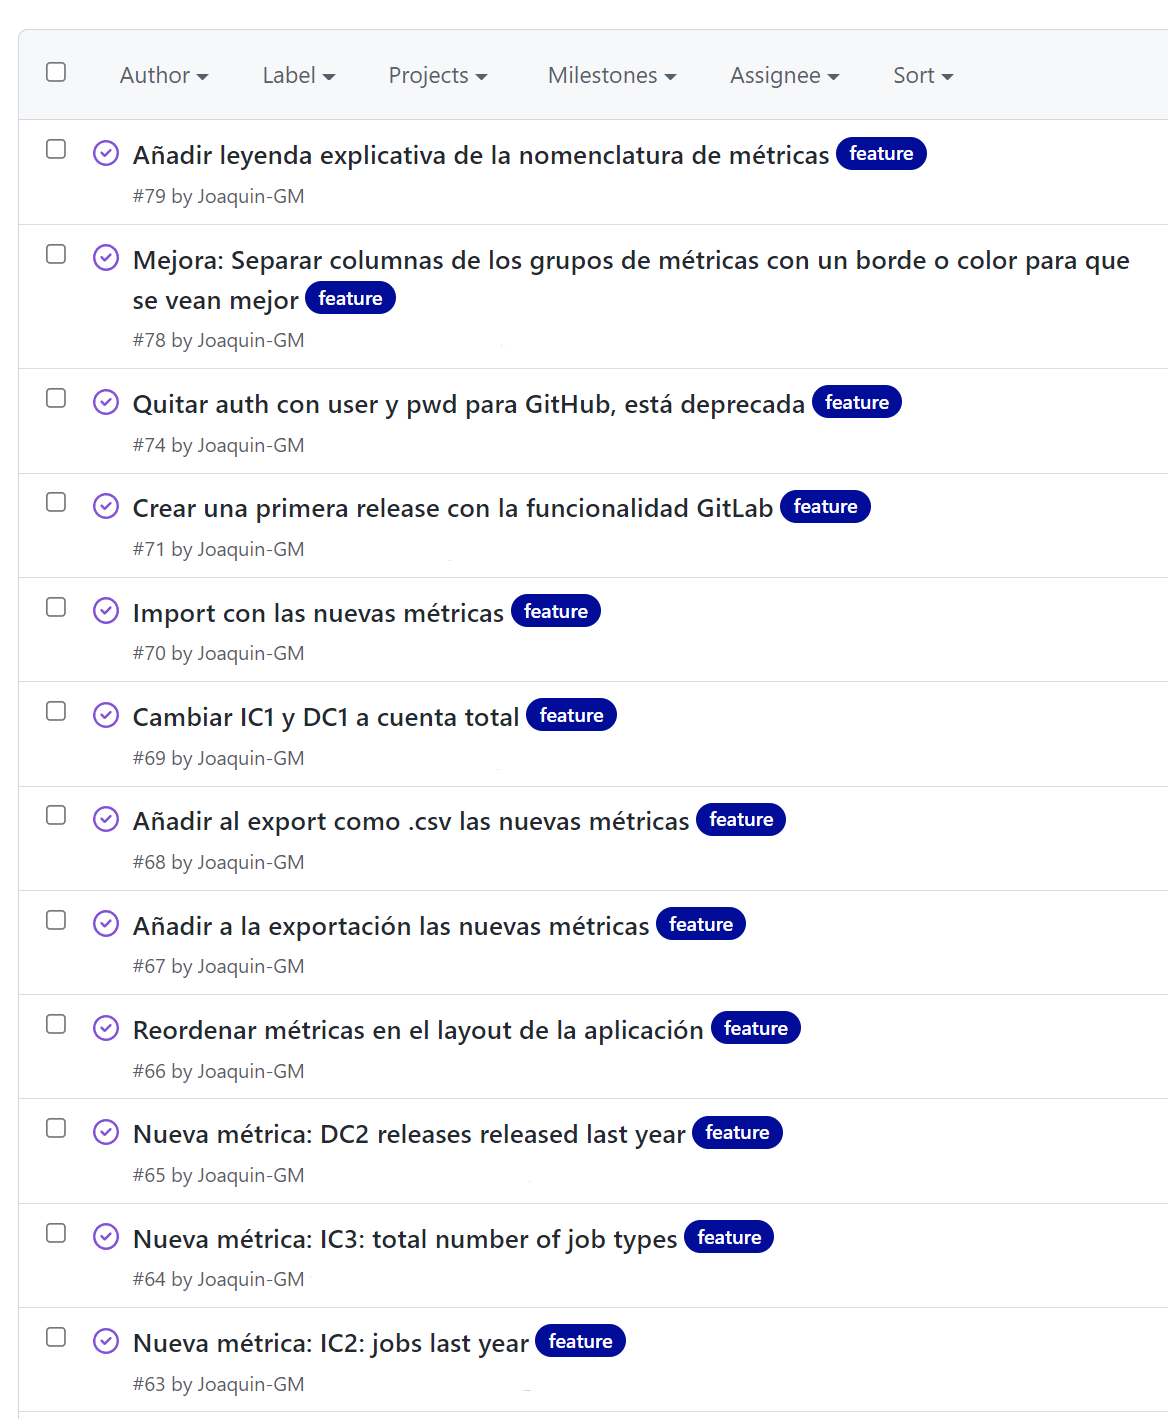
\includegraphics[width=1\textwidth]{AnexA_First_Develop_Issues}
	\caption{\textit{Issues} de desarrollo 1/2}
	\label{fig:AnexA_First_Develop_Issues}
\end{figure}
\FloatBarrier

\begin{figure}[!h]
	\centering
	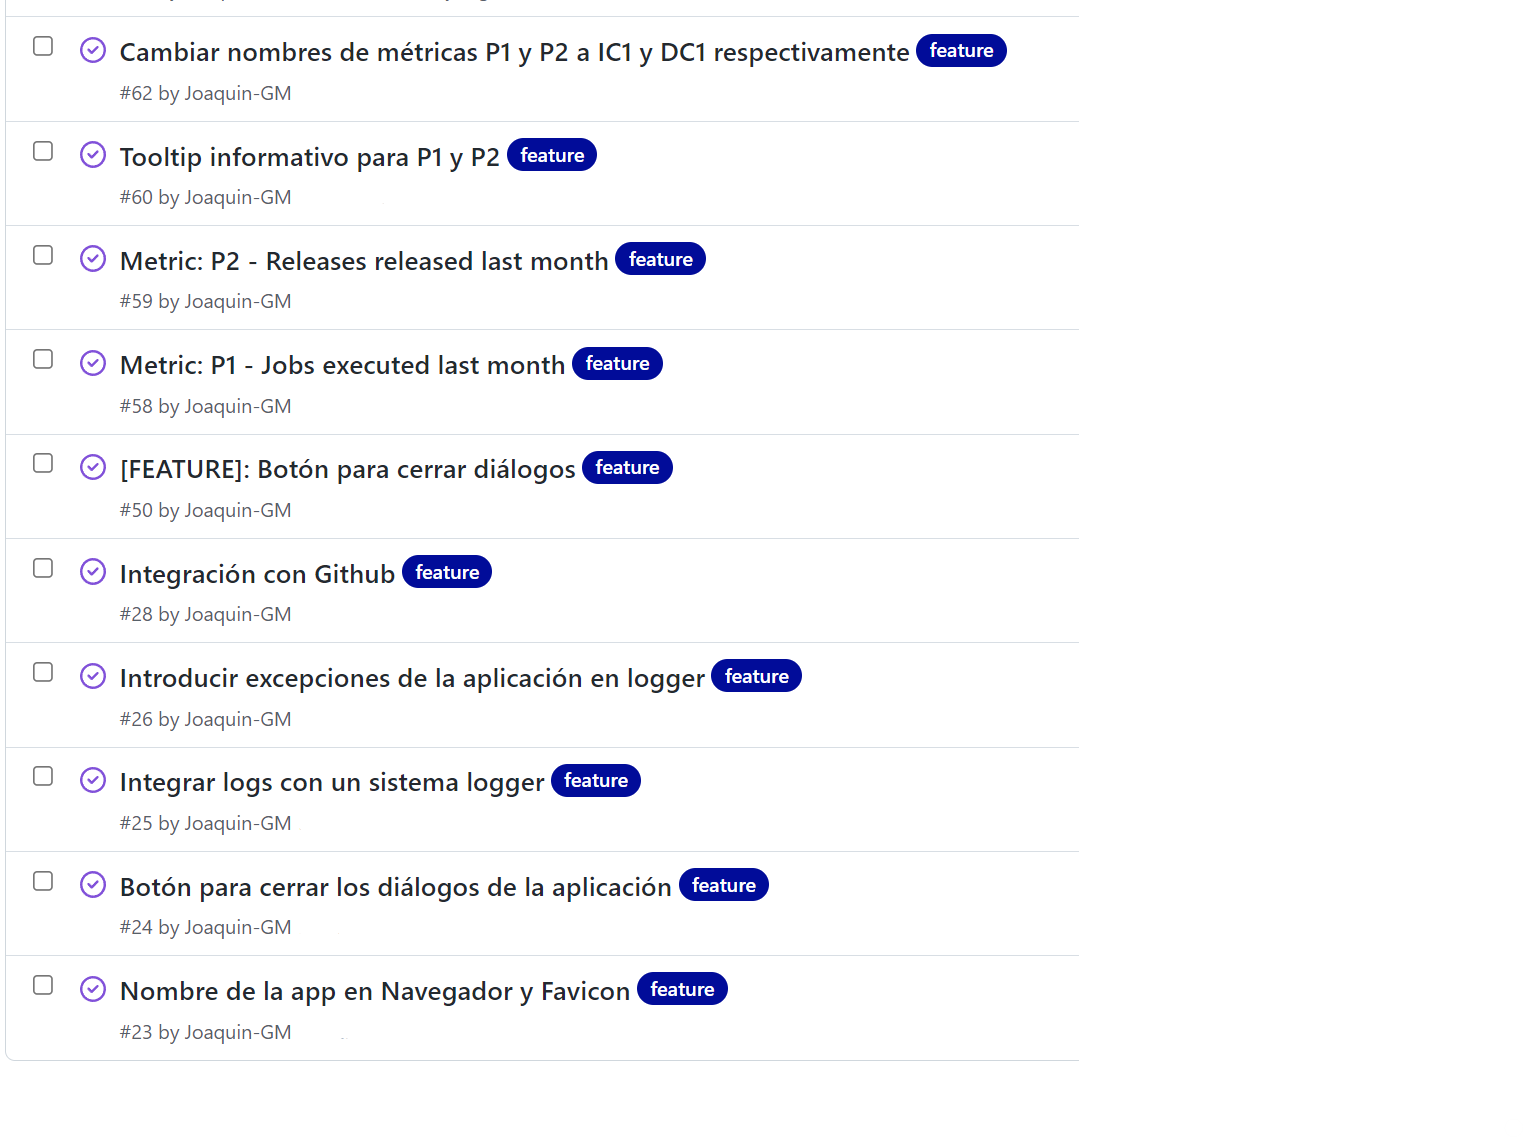
\includegraphics[width=1\textwidth]{AnexA_Second_Develop_Issues}
	\caption{\textit{Issues} de desarrollo 2/2}
	\label{fig:AnexA_Second_Develop_Issues}
\end{figure}
\FloatBarrier

Un ejemplo de gráfico \textit{burndown} de uno de los \textit{sprints} de esta fase puede verse en la figura \ref{fig:AnexA-Develop_BurnDown}

\begin{figure}[!h]
	\centering
	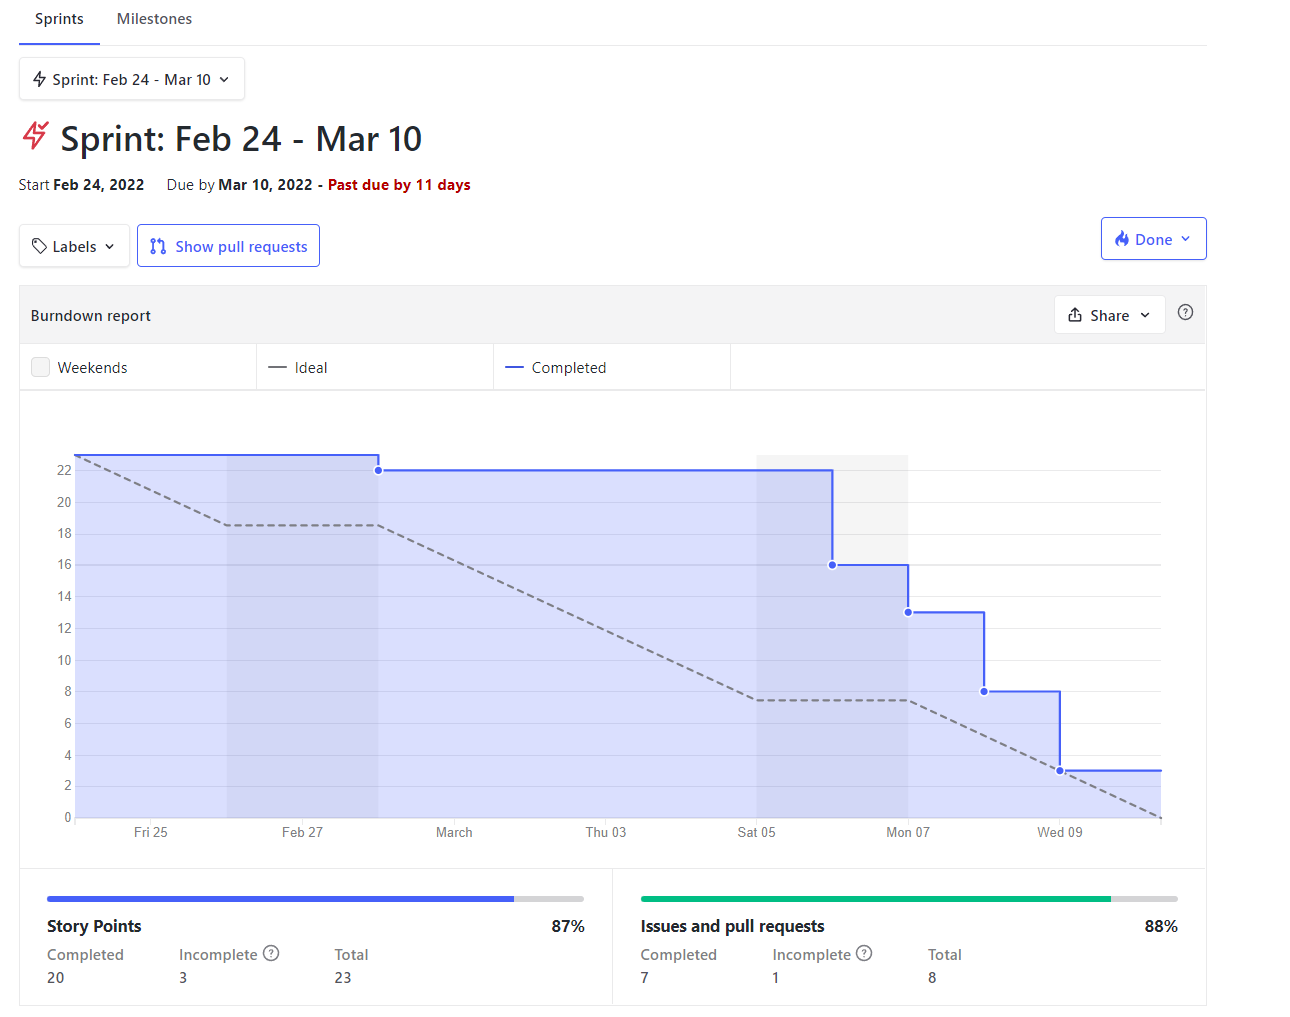
\includegraphics[width=1\textwidth]{AnexA-Develop_BurnDown}
	\caption{\textit{Burndown} de un \textit{sprint} de desarrollo}
	\label{fig:AnexA-Develop_BurnDown}
\end{figure}
\FloatBarrier

En este caso se puede observar que sí se completaron todas las \textit{issues} menos una. Se puede apreciar en el gráfico que durante los primeros días del \textit{sprint} no se pudo terminar ninguna \textit{issue}, si se hubiera podido conseguir nos habríamos aproximado más al avance ideal y probablemente se hubiera podido cerrar la \textit{issue} pendiente de ese sprint.

\subsubsection{Segunda fase de documentación}
En esta última fase de documentación se trabajó durante 2 \textit{sprint} (4 semanas) en los siguientes apartados:

\begin{itemize}
	\item Memoria: Aspectos relevantes del desarrollo del proyecto
	\item Memoria: Trabajos relacionados
	\item Memoria: Conclusiones y líneas de trabajo futuras
	\item Anexos
	\item Vídeos de presentación del proyecto
\end{itemize}

A continuación podemos ver las \textit{issues} con las que se trabajó en esta fase:

\begin{figure}[!h]
	\centering
	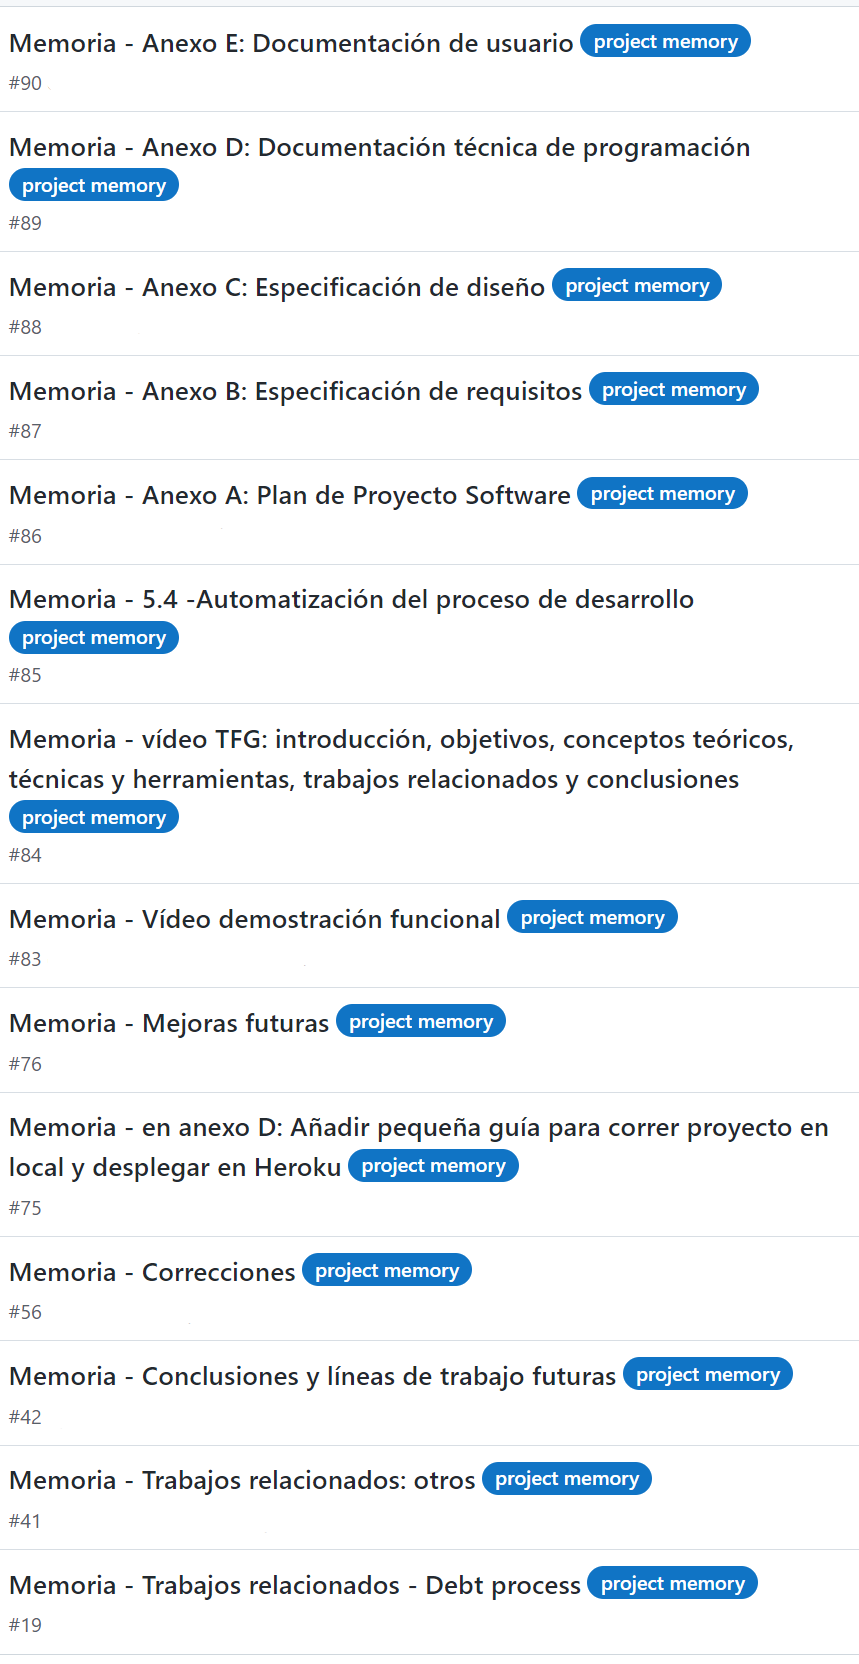
\includegraphics[width=0.7\textwidth]{AnexA_Second_Memory_Issues}
	\caption{Últimas \textit{issues} relacionadas con la memoria, anexos y documentación}
	\label{fig:AnexA_Second_Memory_Issues}
\end{figure}
\FloatBarrier

Un último ejemplo de gráfico \textit{burndown} de esta fase en el que sí se fue avanzando siguiendo el avance ideal:

\begin{figure}[!h]
	\centering
	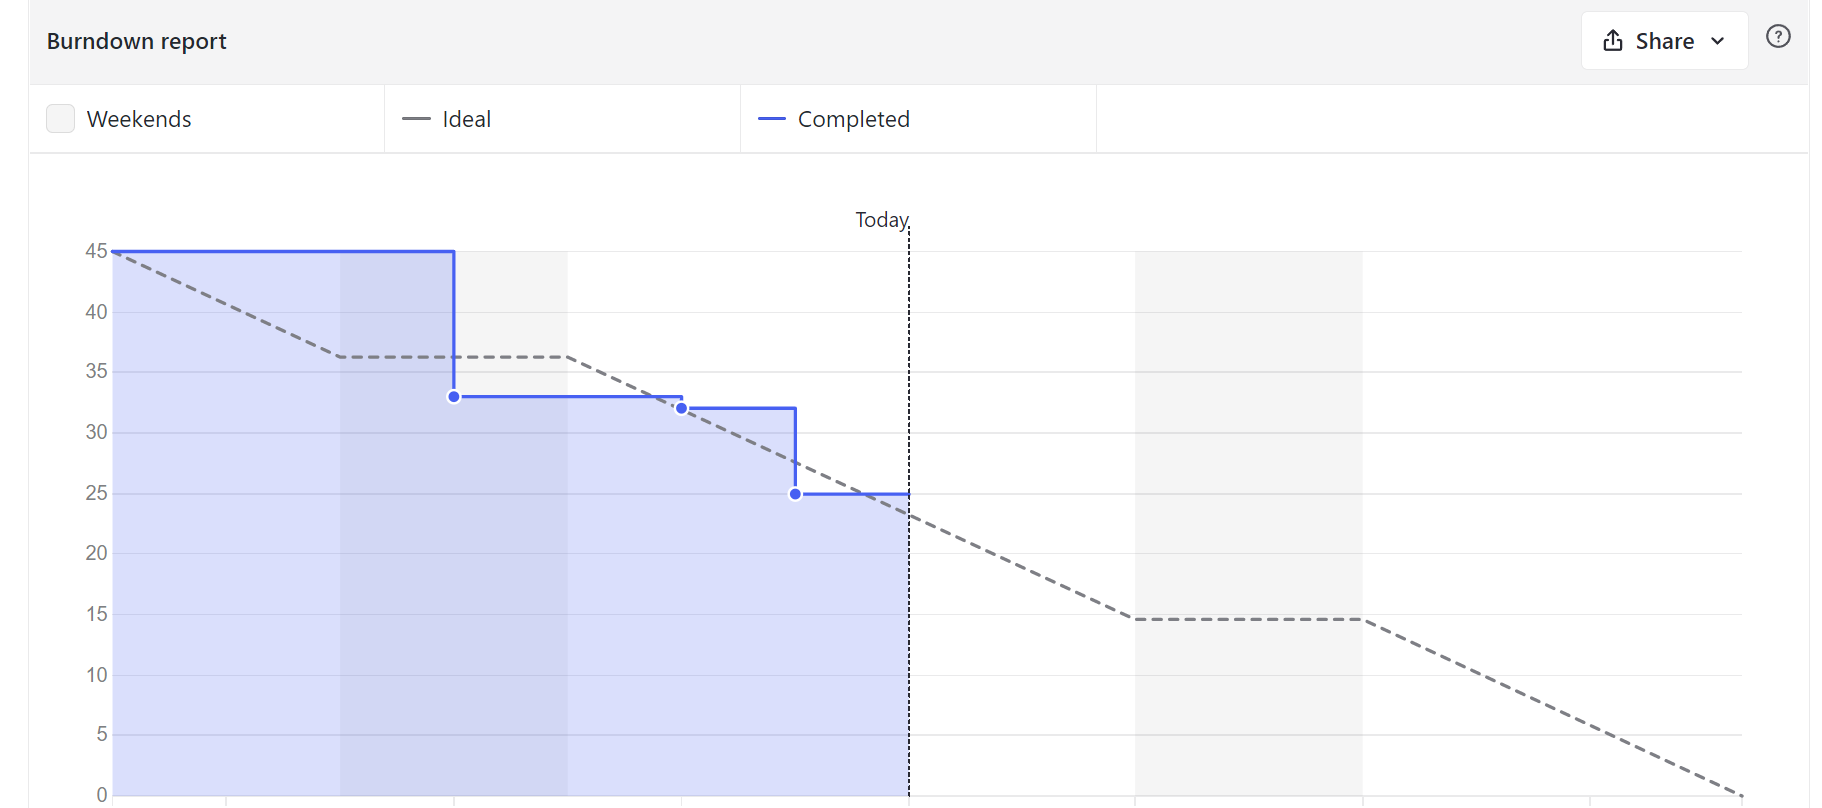
\includegraphics[width=1\textwidth]{AnexA-Second_Memory_BurnDown}
	\caption{\textit{Burndown} del último \textit{sprint} de documentación}
	\label{fig:AnexA-Second_Memory_BurnDown}
\end{figure}
\FloatBarrier


\section{Estudio de viabilidad}
\subsection{Viabilidad económica}
A continuación se va a realizar un estudio del coste que supondría haber realizado el proyecto en un entorno real y se analizan posibles maneras de monetizar el proyecto para cubrir este coste.

\subsubsection{Costes}
\textbf{Costes de personal}

Es el mayor de los costes como en prácticamente todos los proyectos de desarrollo de software, el proyecto ha sido realizado por una persona con una jornada reducida de unas 12 horas semanales (debido a la simultaneidad del desarrollo del proyecto con la actividad laboral del alumno) durante 8 meses (mediados de octubre 2021 hasta mediados de junio de 2022). Se pueden estimar los siguientes valores:
\begin{itemize}
	\tightlist
	\item Salario neto mensual: 500 \officialeuro
	\item Retención por IRPF de carácter general del 15\% \cite{agencia_tributaria_cuadro_2022}
	\item Una retribución a la Seguridad Social de 28,3\% \cite{ministerio_de_empleo_y_seguridad_social_bases_2022}: Empresa (23,6\%) +  Trabajador(Desempleo de tipo general + FOGASA + Formación profesional)(4,70\%)
\end{itemize}

Realizando cálculos, se obtiene:
\begin{longtable}[]{@{}lr@{}}
	\toprule
	\begin{minipage}[b]{0.38\columnwidth}\raggedright\strut
		\textbf{Concepto}\strut
	\end{minipage} & \begin{minipage}[b]{0.40\columnwidth}\raggedright\strut
		\textbf{Coste}\strut
	\end{minipage}\tabularnewline
	\midrule
	\endhead
	\begin{minipage}[t]{0.38\columnwidth}\raggedright\strut
		Salario mensual neto\strut
	\end{minipage} & \begin{minipage}[t]{0.40\columnwidth}\raggedright\strut
		500 \officialeuro (12h/semana)\strut
	\end{minipage}\tabularnewline
	\begin{minipage}[t]{0.38\columnwidth}\raggedright\strut
		Retención IRPF (15\%)\strut
	\end{minipage} & \begin{minipage}[t]{0.40\columnwidth}\raggedright\strut
		122,15 \officialeuro\strut
	\end{minipage}\tabularnewline
	\begin{minipage}[t]{0.38\columnwidth}\raggedright\strut
		Seguridad Social (29,9\%)\strut
	\end{minipage} & \begin{minipage}[t]{0.40\columnwidth}\raggedright\strut
		192,18 \officialeuro\strut
	\end{minipage}\tabularnewline
	\begin{minipage}[t]{0.38\columnwidth}\raggedright\strut
		Salario mensual bruto\strut
	\end{minipage} & \begin{minipage}[t]{0.40\columnwidth}\raggedright\strut
		814,33 \officialeuro\strut
	\end{minipage}\tabularnewline
	\midrule
	\begin{minipage}[t]{0.38\columnwidth}\raggedright\strut
		\textbf{Total 8 meses}\strut
	\end{minipage} & \begin{minipage}[t]{0.40\columnwidth}\raggedright\strut
		4.314,33 \officialeuro\strut
	\end{minipage}\tabularnewline
	\bottomrule
	\caption{Costes de personal}
\end{longtable}

\textbf{Costes de hardware}

Se va a considerar como coste únicamente un ordenador, hay que tener en cuenta que el período de amortización de equipos para procesos de información es de 8 años \cite{agencia_tributaria_tabla_2022}, que se considera un coste de 800 \officialeuro \thinspace para dicho ordenador y que se ha usado durante 8 meses:

\begin{longtable}[]{@{}lrr@{}}
	\toprule
	\begin{minipage}[b]{0.29\columnwidth}\raggedright\strut
		\textbf{Concepto}\strut
	\end{minipage} & \begin{minipage}[b]{0.18\columnwidth}\raggedright\strut
		\textbf{Coste}\strut
	\end{minipage} & \begin{minipage}[b]{0.32\columnwidth}\raggedright\strut
		\textbf{Coste amortizado}\strut
	\end{minipage}\tabularnewline
	\midrule
	\endhead
	\begin{minipage}[t]{0.29\columnwidth}\raggedright\strut
		Ordenador portátil\strut
	\end{minipage} & \begin{minipage}[t]{0.18\columnwidth}\raggedright\strut
		800 \officialeuro\strut
	\end{minipage} & \begin{minipage}[t]{0.32\columnwidth}\raggedright\strut
		66,67 \officialeuro\strut
	\end{minipage}\tabularnewline
	\midrule
	\begin{minipage}[t]{0.29\columnwidth}\raggedright\strut
		\textbf{Total}\strut
	\end{minipage} & \begin{minipage}[t]{0.18\columnwidth}\raggedright\strut
		800 \officialeuro\strut
	\end{minipage} & \begin{minipage}[t]{0.32\columnwidth}\raggedright\strut
		66,67 \officialeuro\strut
	\end{minipage}\tabularnewline
	\bottomrule
	\caption{Costes de hardware}
\end{longtable}

\textbf{Costes de software}

Todo el software empleado para el desarrollo del proyecto tiene licencias gratuitas, salvo el propio sistema operativo. Se ha utilizado \textit{Windows 11} en este caso y se ha trabajado con una licencia que tiene un coste muy reducido de unos 12 \officialeuro al ser una clave \textit{OEM} (que son perfectamente legales).\\
Teniendo en cuenta dicho coste y que la amortización para sistemas y programas informáticos es de 6 años \cite{agencia_tributaria_tabla_2022} y se ha utilizado durante 8 meses:

\begin{longtable}[]{@{}lrr@{}}
	\toprule
	\begin{minipage}[b]{0.29\columnwidth}\raggedright\strut
		\textbf{Concepto}\strut
	\end{minipage} & \begin{minipage}[b]{0.18\columnwidth}\raggedright\strut
		\textbf{Coste}\strut
	\end{minipage} & \begin{minipage}[b]{0.32\columnwidth}\raggedright\strut
		\textbf{Coste amortizado}\strut
	\end{minipage}\tabularnewline
	\midrule
	\endhead
	\begin{minipage}[t]{0.29\columnwidth}\raggedright\strut
		\textit{Windows 10 Home}\strut
	\end{minipage} & \begin{minipage}[t]{0.18\columnwidth}\raggedright\strut
		12 \officialeuro\strut
	\end{minipage} & \begin{minipage}[t]{0.32\columnwidth}\raggedright\strut
		1,33 \officialeuro\strut
	\end{minipage}\tabularnewline
	\midrule
	\begin{minipage}[t]{0.29\columnwidth}\raggedright\strut
		\textbf{Total}\strut
	\end{minipage} & \begin{minipage}[t]{0.18\columnwidth}\raggedright\strut
		12 \officialeuro\strut
	\end{minipage} & \begin{minipage}[t]{0.32\columnwidth}\raggedright\strut
		1,33 \officialeuro\strut
	\end{minipage}\tabularnewline
	\bottomrule
	\caption{Costes de software}
\end{longtable}

\textbf{Otros costes}
Se van a tener en cuenta además otros costes necesarios para poder desarrollar el proyecto en un entorno real. Se va a considerar una opción algo pesimista en la que es necesario alquilar una oficina para el desarrollador con sus costes asociados durante los 8 meses de desarrollo (alquiler unos 50 \officialeuro al mes, internet unos 30 \officialeuro al mes y algo de material de oficina):\\

\begin{longtable}[]{@{}lr@{}}
	\toprule
	\begin{minipage}[b]{0.48\columnwidth}\raggedright\strut
		\textbf{Concepto}\strut
	\end{minipage} & \begin{minipage}[b]{0.18\columnwidth}\raggedright\strut
		\textbf{Coste}\strut
	\end{minipage}\tabularnewline
	\midrule
	\endhead
	\begin{minipage}[t]{0.48\columnwidth}\raggedright\strut
		Alquiler de oficina\strut
	\end{minipage} & \begin{minipage}[t]{0.18\columnwidth}\raggedright\strut
		400 \officialeuro\strut
	\end{minipage}\tabularnewline
	\begin{minipage}[t]{0.48\columnwidth}\raggedright\strut
		Internet\strut
	\end{minipage} & \begin{minipage}[t]{0.18\columnwidth}\raggedright\strut
		240 \officialeuro\strut
	\end{minipage}\tabularnewline
	\begin{minipage}[t]{0.48\columnwidth}\raggedright\strut
		Material de oficina\strut
	\end{minipage} & \begin{minipage}[t]{0.18\columnwidth}\raggedright\strut
		40 \officialeuro\strut
	\end{minipage}\tabularnewline
	\midrule
	\begin{minipage}[t]{0.48\columnwidth}\raggedright\strut
		\textbf{Total}\strut
	\end{minipage} & \begin{minipage}[t]{0.18\columnwidth}\raggedright\strut
		680 \officialeuro\strut
	\end{minipage}\tabularnewline
	\bottomrule
	\caption{Costes varios.}
\end{longtable}

\textbf{Coste total}

El coste total por tanto sería:\\

\begin{longtable}[]{@{}lr@{}}
	\toprule
	\begin{minipage}[b]{0.22\columnwidth}\raggedright\strut
		\textbf{Concepto}\strut
	\end{minipage} & \begin{minipage}[b]{0.22\columnwidth}\raggedright\strut
		\textbf{Coste}\strut
	\end{minipage}\tabularnewline
	\midrule
	\endhead
	\begin{minipage}[t]{0.22\columnwidth}\raggedright\strut
		Personal\strut
	\end{minipage} & \begin{minipage}[t]{0.22\columnwidth}\raggedright\strut
		4.314,33 \officialeuro\strut
	\end{minipage}\tabularnewline
	\begin{minipage}[t]{0.22\columnwidth}\raggedright\strut
		Hardware\strut
	\end{minipage} & \begin{minipage}[t]{0.22\columnwidth}\raggedright\strut
		66,67 \officialeuro\strut
	\end{minipage}\tabularnewline
	\begin{minipage}[t]{0.22\columnwidth}\raggedright\strut
		Software\strut
	\end{minipage} & \begin{minipage}[t]{0.22\columnwidth}\raggedright\strut
		1,33 \officialeuro\strut
	\end{minipage}\tabularnewline
	\begin{minipage}[t]{0.22\columnwidth}\raggedright\strut
		Otros\strut
	\end{minipage} & \begin{minipage}[t]{0.22\columnwidth}\raggedright\strut
		680 \officialeuro\strut
	\end{minipage}\tabularnewline
	\midrule
	\begin{minipage}[t]{0.22\columnwidth}\raggedright\strut
		Total\strut
	\end{minipage} & \begin{minipage}[t]{0.22\columnwidth}\raggedright\strut
		5.062,33 \officialeuro\strut
	\end{minipage}\tabularnewline
	\bottomrule
	\caption{Costes totales.}
\end{longtable}

\subsubsection{Beneficios}

Actualmente la aplicación tiene licencia libre y es gratuita por lo que no se obtiene ningún beneficio con ella. Para poder obtenerlos se pueden plantear diferentes alternativas:

\begin{itemize}
	\item Pago a través de licencias de uso.
	\item Pago por subscripción al servicio.
	\item Incluir publicidad, esta solución podría ser la mejor si queremos cubrir costes y que el proyecto siga siendo de uso gratuito.
\end{itemize}


\subsection{Viabilidad legal}
Nuestro software al trabajar con repositorios públicos o aquellos a los que el usuario tenga acceso no puede incumplir con la privacidad de los mismos, por tanto, lo que hay que analizar son las licencias del software que se ha usado durante desarrollo de la aplicación.\\
 En la Fig. \ref{fig:AnexA_Licencias} podemos ver los artefactos utilizados en el proyecto (dependencias del proyecto en el fichero \ruta{pom.xml}:) y cuya información se puede obtener en el repositorio de \textit{Maven} \footnote{\url{https://mvnrepository.com/}} 

\begin{figure}[!h]
	\centering
	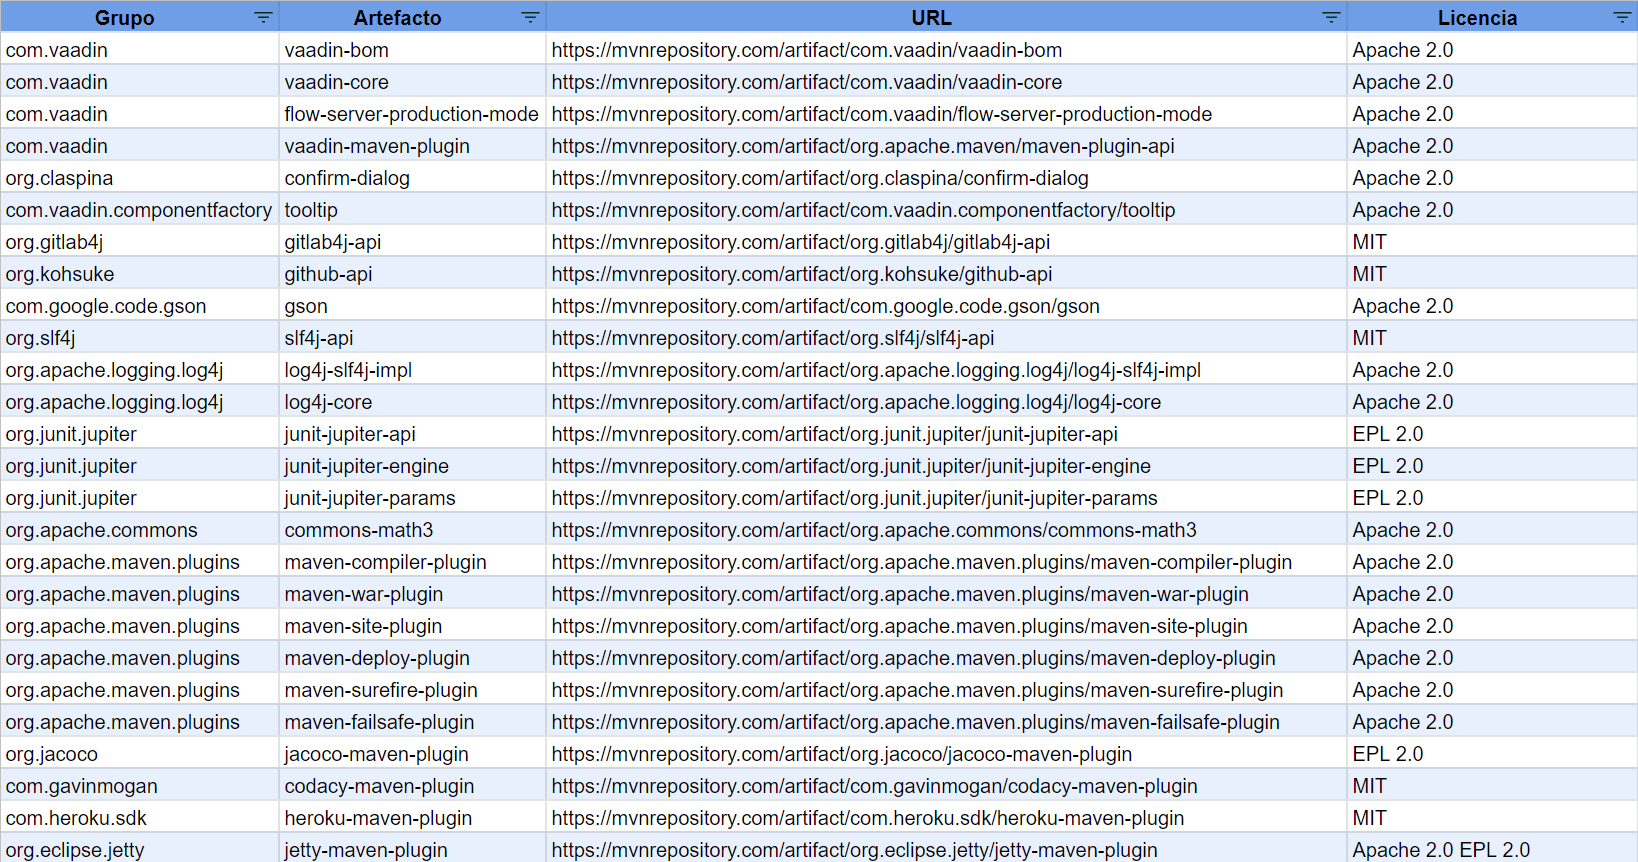
\includegraphics[scale=0.32]{AnexA_Licencias}
	\caption{Licencias de las dependencias del proyecto}
	\label{fig:AnexA_Licencias}
\end{figure}
\FloatBarrier

Por lo tanto, las licencias a las que está sometido nuestro proyecto son, de más a menos permisivas:
\begin{itemize}
	\item \textit{MIT}
	\item \textit{Apache v.2.0}
	\item \textit{EPL 2.0}
\end{itemize}

La licencia más restrictiva de las tres es la \textit{Eclipse Public License} que es la que tienen las librerías que se utilizan para pruebas (JUnit).

A este proyecto se le podría dar la licencia \textit{GNU General Public License v3.0}, que permite el uso comercial, modificación, distribución, uso privado y el uso de patentes mientas queramos que siga siendo de acceso y uso público como hasta hora.
Esta licencia es compatible con las del software utilizado en el proyecto pues la versión \textit{EPL 2.0} permite utilizar la versión 2 de la \textit{GPL} de \textit{GNU} y posteriores como licencia secundaria en una parte especifica del código. Por esto, se garantiza la compatibilidad de ese código con esas versiones de la GPL \cite{santiago_lista_2019}.